\chapter {Introduction}
\label{ch:intro}

\section {Background information}

Extreme precipitation, or heavy rainstorms as sometimes referred, are those that happen very rarely. They account for a considerable part of annual precipitation at a given location. From the perspective of magnitude, heavy storms are defined using the hourly rainrate of 7.6mm/hr [\textit{Huschke}, 1959].

Over the past century, numerous water infrastructures have been built to serve the water-related need of people worldwide [\textit{Mitchell}, 1990]. Those larger ones often serve multiple purposes, such as agriculture, navigation, hydropower, and flooding control. Failure of such high-hazard dams would bring catastrophic eco-societal loss. Therefore, they are often the center of local and regional water resources management [\textit{Asmal and Coauthors}, 2000; \textit{Grigg}, 1996]. For example, the failure of the South Fork dam in Pennsylvania, USA in 1889 caused 2,209 deaths and an economic loss of 17 million dollars [\textit{Frank}, 1988; \textit{VandenBerge et al.}, 2011].  For these infrastructures, Probable Maximum Precipitation (PMP), or Probable Maximum Flood (PMF) which can be derived from PMP,  has been widely used to ensure its safety under the extreme weather conditions [\textit{Hossain et al.}, 2012]. PMP is also a widely used design criteria for the nuclear water disposal sites, as any leakage from the failure of site/equipment is not tolerable [\textit{Hayes et al.}, 2015].

Probable Maximum Precipitation (PMP) follows an idea of creating an extreme scenario that covers all the possibilities. In the engineering practice, the definition by the World Meteorological Organization (WMO) is often adopted: probable maximum precipitation is the ``theoretical maximum precipitation that a given watershed can receive in a given duration of time''. Besides this definition, WMO also gives detailed instructions on how to make PMP estimation using various approaches [\textit{World Meteorological Organization (WMO)}, 1986]. In general, they can be classified into: local method (maximization of local storms), transposition method (storm transposition from same climatological regions), generalized method (based on some provided PMP distribution maps), as well as statistical method such as the one proposed in \textit{Hershfield} [1965]. At the national scale, different countries adopt different methods for their own PMP estimation. For example, PMP in India follows the generalized PMP approach [\textit{Rakhecha and Kennedy}, 1995; \textit{Rakhecha and Singh}, 2009], with the adjustment carried for the impact of local topography. In the US, moisture maximization method is chosen by NOAA as the standard approach, and NOAA has published a series of instructions for different climatological regions, now known as HydroMeteorological Reports (HMRs).

The moisture maximization approach estimates PMP as equation \ref{eq:1-1}, where $P$ is the observed precipitation, $PW$ is the observed maximum 12-hour persisting precipitable water in the storm duration, and $PWm$ is the climatological 12-hour persisting precipitable water at this location. In practice, $PW$ and $PWm$ are estimated from surface dew point temperature measurement, assuming a pseudoadiabatic air condition. From long-term ground observations, the most severe rainstorms in the history are maximized following this equation, and the maximum of these derived values are defined as the PMP of this site. At certain HMR regions where surface topography plays important roles in the storming process (such as the watersheds along the west coast), the topographic adjustment is applied as appropriate.

\begin{equation}
PMP = P \times{\frac{PWm}{PW}}
\label{eq:1-1}
\end{equation}

In the recent decades, this moisture maximization approach has been revisited with high-quality observation and advanced atmospheric modeling. For example, \textit{Abbs} [1999] used atmospheric model and checked the linear assumption assumed in equation \ref{eq:1-1}. This study found that such linear assumption may introduce bias in the maximization procedure. On the other hand, the storm efficiency during the observed extreme precipitation events are often between 80\% and 100\%. Thus the moisture maximization does not fully release the precipitation potential. \textit{Chen and Bradley} [2006] analyzed observation data and concluded that surface dew point temperature plus pseudoadiabatic assumption tend to overestimate $PW$ of the air column.

As a response to these concerns, numerical modeling has been proposed as an alternative to the traditional approach. As a basis of model-based PMP estimation, model reconstruction of extreme precipitation has demonstrated its capability across various extreme rainfall events across the world in the past several decades [\textit{Kato}, 1998; \textit{Rao et al.}, 2007; \textit{Vaidya and Kulkarni}, 2007; \textit{Kumar et al.}, 2008; \textit{Chang et al.}, 2009; \textit{Pennelly et al.}, 2014; \textit{Li et al.}, 2017; \textit{Yang et al.}, 2017]. With good quality input data (i.e., initial and boundary conditions to the simulation), modern atmospheric models can reconstruct the spatial-temporal rainfall pictures in the context of various weather systems (e.g., atmospheric rivers, cyclones/tornadoes, mesoscale convective systems, topographic precipitation). Along with high-quality rainfall pictures, models also provide complete information on the related meteorological diagnostic variables (such as air temperature, wind fields, and precipitable water as used in equation \ref{eq:1-1}). Numerical models do not require ground observation data as direct input (though ground observation is highly useful in the data assimilation procedures that generate the input to these numerical models). Therefore it is capable of reconstructing the extreme events since the 1940s given the current availability of model input datasets. Several other datasets, such as the 20th century reanalysis products (20CRs), even enable us to look into the weather events of as early as the 1850s. They potentially provide more complete datasets of extreme events and more quality-consistent data of precipitation/diagnostic variables as compared with ground observations on the scale of centuries. There have been studies checking the data quality of the 20CRs, as well as modeling efforts on the storms as old as in the 1960s [\textit{Yang et al.}, 2017]. However, up to now, no studies have been done to quantify the usability of these datasets in the extreme event simulations for the early periods (before the 1940s or even the 1900s).

As the science/engineering communities get concerned with the ongoing climate change in the recent decades, atmospheric models with climate projections can also reveal the future of the extreme events under climate change. For example, \textit{Warner et al.}, 2015 looked into the extreme precipitation in the US Pacific Northwest region duirng 1970-2000 and 2070-2100 using CMIP5 models, and found that precipitable water (the moisture source of precipitation) is going to increase by 15\% to 39\% in the future. Kunkel et al. [2013] used CMIP5 results to investigate the PMP in the future, and found that both moisture avaibility and atmospheric vertical winds would increase in the future, suggesting a potential increase of PMPs. Study by \textit{Rastogi et al.} [2017] took this approach further and investigated the possible change of PMP design standard in the Alabama-Coosa-Tallapoosa river basin in the southeast US.

Based on good constructions of extreme precipitation events, a number of ways to modify the model and make model-based PMP estimations have been proposed. In general, these approaches can be classified into 3 categories: 1) disturbance of air moisture through changing air temperature/relative humidity and keeping the atmospheric columns throughout the simulation domain fully moist during the storm events [\textit{Ohara et al.}, 2011; \textit{Tan}, 2010]; 2) disturbance of moisture flux through changing wind speed or wind fields [\textit{Ishida et al.}, 2015]; 3) combination of worst historical environmental conditions [\textit{Tan}, 2010]. However, all these studies are based on the ``trail and error'', and the largest maximized precipitation amount is taken then as PMP value. Since there has been no comprehensive study to date that investigates the key atmospheric conditions that affect extreme storms (e.g., moisture availability, atmospheric instability, large-scale convergence), the engineering community is still left without a rational guideline on the use of numerical models for PMP estimation. In other words, studies that can derive systematic and detailed guidance as those in HMRs are required.

In summary, for the engineers to complete the switch to the model-based PMP estimation approach, the following challenges need to be addressed:

1. Unlike land surface hydrological modeling, atmospheric models usually involve parameterization schemes to approximate the atmospheric processes (e.g., water phase transition, sub-grid scale convections). Therefore, what would be a good modeling framework that can be easily adopted by engineering for rainfall simulations? What storms can we now confidently construct given the current reanalysis/projection data?

2. Physics-based methods should be developed to estimate PMP in the numerical models. The current trail-based approach needs to be replaced with more physics-based and more convincing approaches that are based on the understanding of storm processes and local climatology.

3. A smooth transition from the traditional approach to the proposed model-based approach is required. There have been thousands of large water infrastructures designed using traditional PMP criteria. Therefore, it is critical that we understand what has changed, while what is kept in the new model-based approaches (figure \ref{fig:1-1}). Only by this way can we connect the model-based PMPs to the safety of existing infrastructures in the future.


\begin{figure}[htbp]
	\centering
	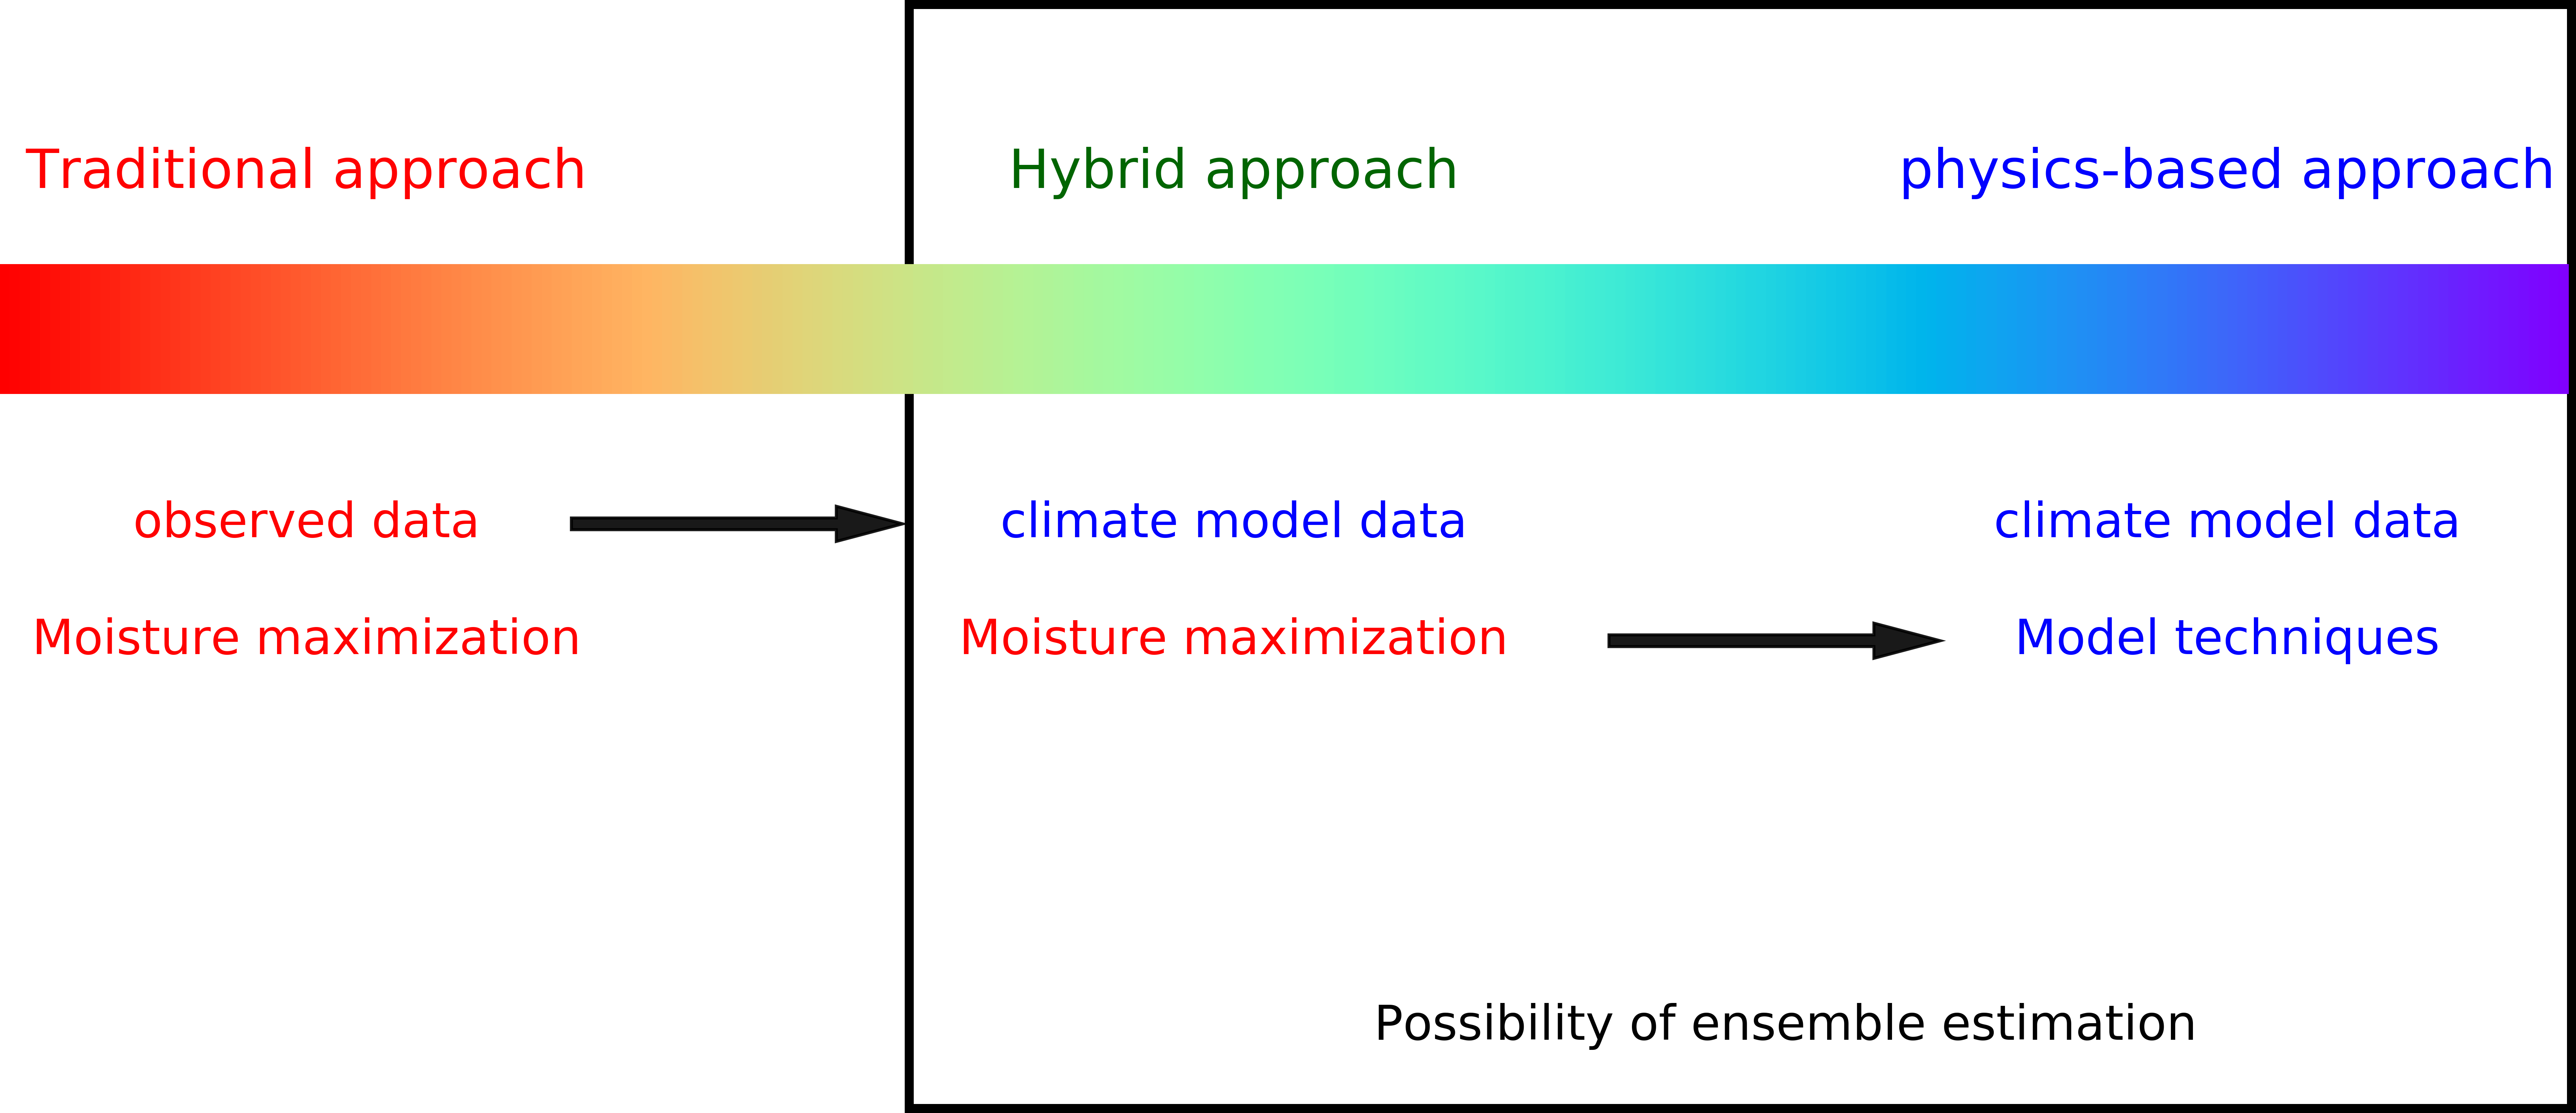
\includegraphics[width=\linewidth]{pics/ch1/fig1.png}
	\caption{A complete transition from traditional approach to physics-based approach of PMP estimation.}
    \label{fig:1-1}
\end{figure}

\section {Objectives}

Through this dissertation, I hope to have a better understanding of the relationship between extreme precipitation and the environmental conditions. Taking this information into atmospheric numerical modeling, I hope to help the engineering community to get ready to utilize numerical model for infrastructure safety evaluation. To be specific, I hope to achieve the following goals:

1. To establish a numerical modeling framework for extreme rainfall event simulation in engineering practice.

2. To develop a method to physically estimate PMP while accounting for uncertainties for engineering practice.

3. To estimate PMP change as a function of the climate change.



\section {Approach}

The core of this dissertation is organized as follows:

Chapter \ref{ch:JHE} presents a numerical modeling framework (based on WRF) for engineering extreme precipitation events investigation. Chapter \ref{ch:EF} takes this framework and examines out capability of reconstructing the extreme precipitation events in the history. These two chapters lay the foundation of model-based storm construction and thus PMP estimation. Chapter \ref{ch:JHM} performs a statistical analysis of the historical extreme precipitation as reflected by the major reanalysis products, and reveals the spatially heterogeneous relationship between extreme precipitation and the environmental conditions. Chapter \ref{ch:WRR} develops the hybrid approach in figure \ref{fig:1-1}, and links the current and proposed PMP estimation approaches. Chapter \ref{ch:con} presents the findings from the collection of research and the recommendations to future studies.